\documentclass[border=10pt]{standalone}
\usepackage[svgnames]{xcolor}
\usepackage{amsmath}
\usepackage{pgfplots}
\pgfplotsset{compat=newest}
\usepackage[sfdefault]{FiraSans}
\usepackage{FiraMono}
\renewcommand*\familydefault{\sfdefault}
\begin{document}
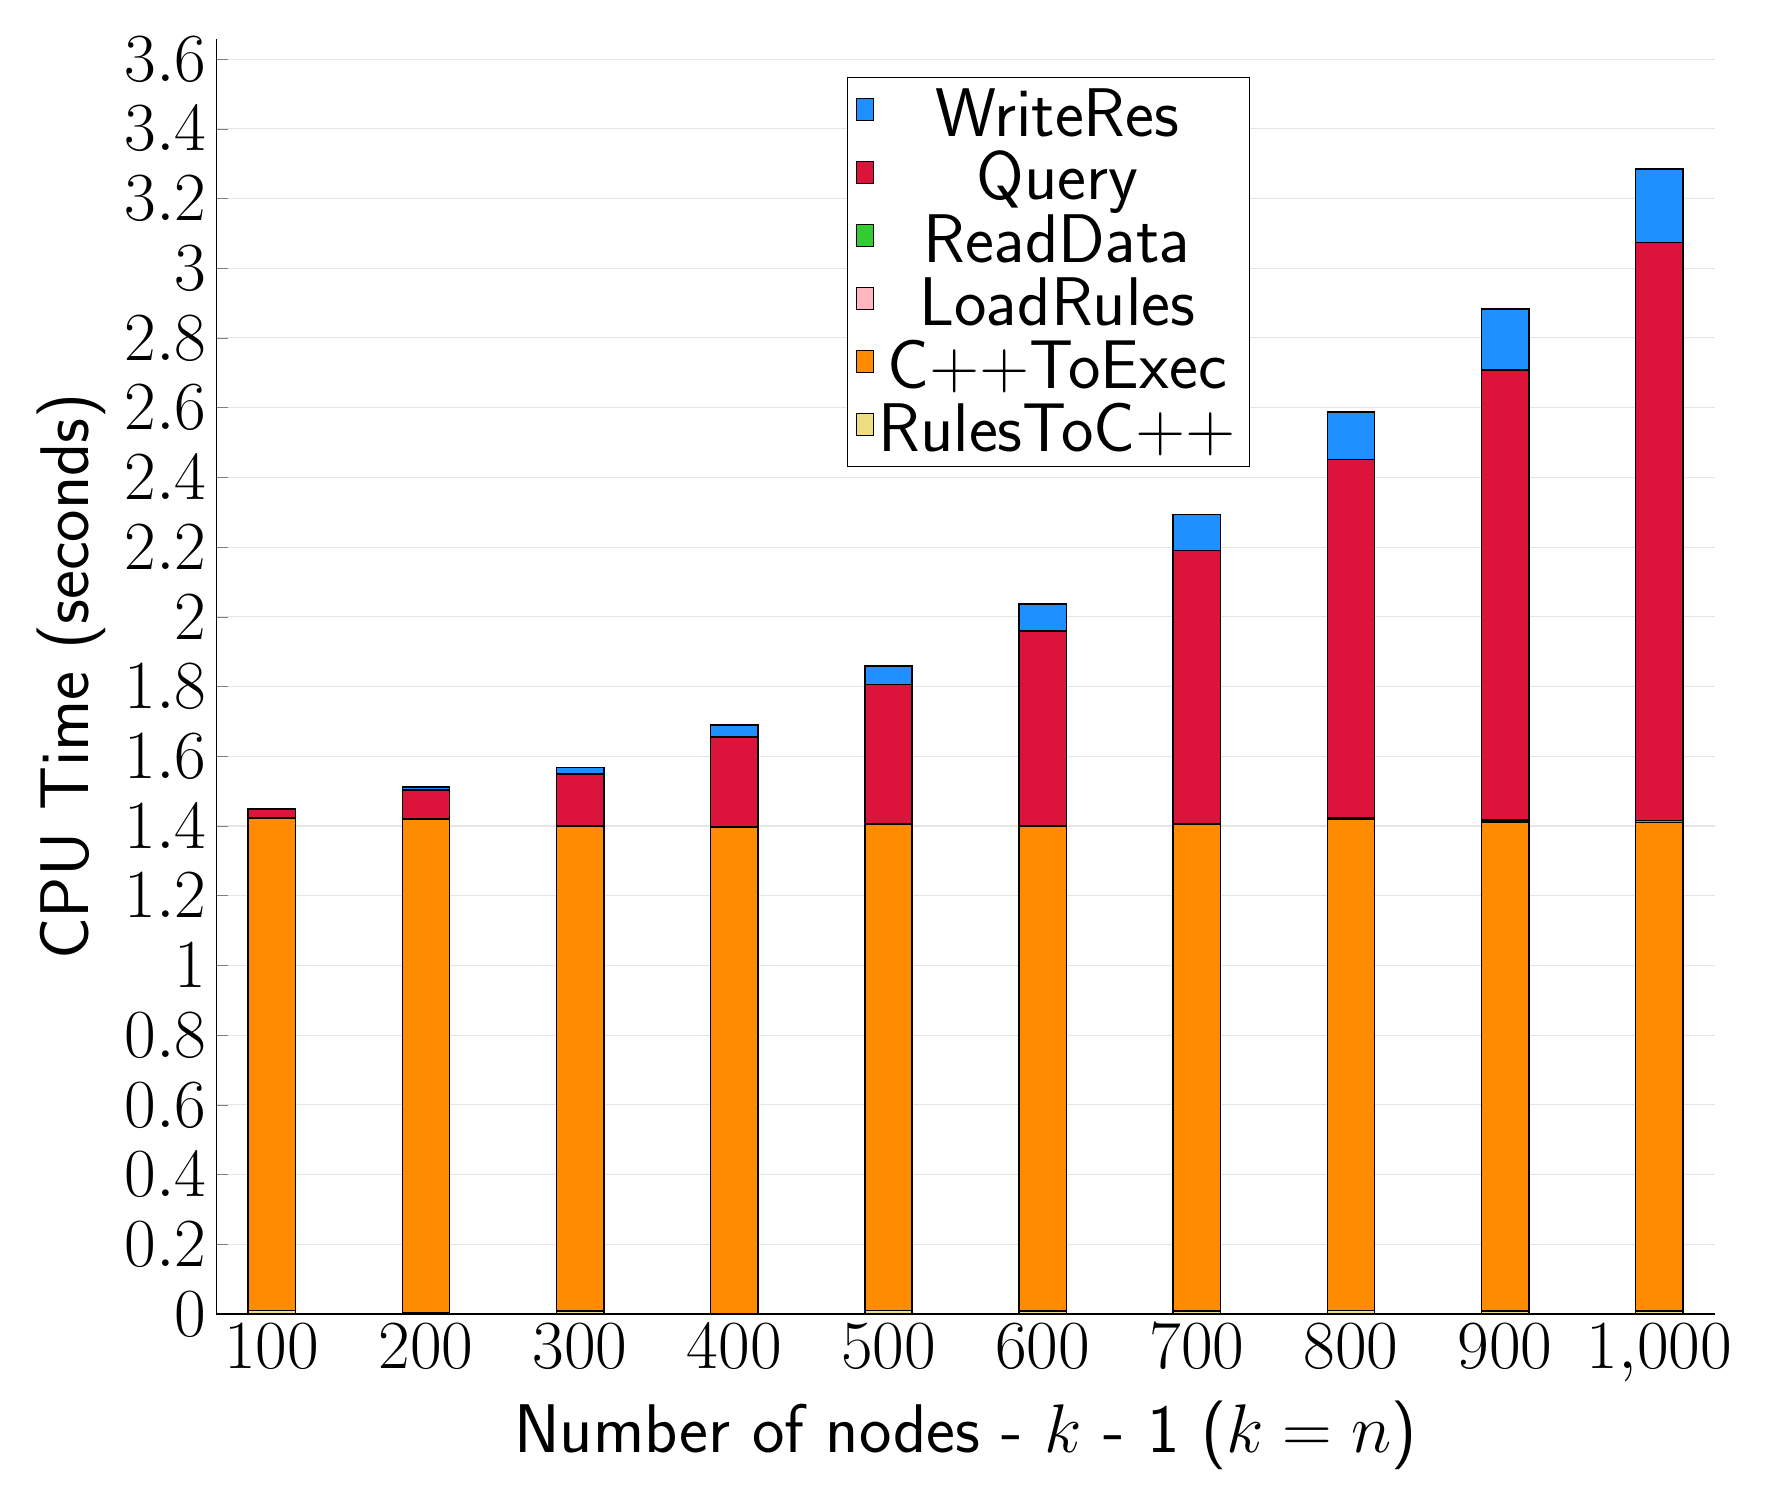
\begin{tikzpicture}
\begin{axis}[
   ybar stacked,
   width=1.7\textwidth,
   bar width=0.6cm,
   ymajorgrids, tick align=inside,
   major grid style={draw=gray!20},
   xtick=data,
   ymin=0, ymax=3.658792,
   axis x line*=bottom,
   axis y line*=left,
   enlarge x limits=0.04,
   legend style={
       at={(0.69, 0.97)},
       anchor=north east,
       legend columns=1,
       font=\Huge,
   },
   ylabel={CPU Time (seconds)},
   xlabel={Number of nodes - $k$ - 1 ($k=n$)},
   label style={font=\Huge},
   tick label style={font=\Huge},
]
\addlegendimage{fill=DodgerBlue, draw=black, line width=0.2pt}
\addlegendentry{WriteRes}
\addlegendimage{fill=Crimson, draw=black, line width=0.2pt}
\addlegendentry{Query}
\addlegendimage{fill=LimeGreen, draw=black, line width=0.2pt}
\addlegendentry{ReadData}
\addlegendimage{fill=LightPink, draw=black, line width=0.2pt}
\addlegendentry{LoadRules}
\addlegendimage{fill=DarkOrange, draw=black, line width=0.2pt}
\addlegendentry{C++ToExec}
\addlegendimage{fill=LightGoldenrod, draw=black, line width=0.2pt}
\addlegendentry{RulesToC++}
\addplot +[fill=LightGoldenrod, draw=black, line width=0.55pt] coordinates {
(100, 0.009999999999999995)
(200, 0.003999999999999998)
(300, 0.007999999999999997)
(400, 0.001999999999999999)
(500, 0.009999999999999995)
(600, 0.007999999999999997)
(700, 0.007999999999999997)
(800, 0.009999999999999995)
(900, 0.007999999999999997)
(1000, 0.007999999999999997)
};
\addplot +[fill=DarkOrange, draw=black, line width=0.55pt] coordinates {
(100, 1.4120000000000001)
(200, 1.4160000000000001)
(300, 1.3920000000000001)
(400, 1.3940000000000001)
(500, 1.394)
(600, 1.3900000000000001)
(700, 1.3960000000000001)
(800, 1.4100000000000004)
(900, 1.4040000000000004)
(1000, 1.4020000000000001)
};
\addplot +[fill=LightPink, draw=black, line width=0.55pt] coordinates {
(100, 0.00011419999999999998)
(200, 0.000149)
(300, 8.56e-05)
(400, 0.00014759999999999998)
(500, 8.34e-05)
(600, 0.000108)
(700, 0.0001216)
(800, 0.00014780000000000001)
(900, 0.000138)
(1000, 0.0001026)
};
\addplot +[fill=LimeGreen, draw=black, line width=0.55pt] coordinates {
(100, 0.0008506)
(200, 0.0014746)
(300, 0.0017418)
(400, 0.0025889999999999997)
(500, 0.0021608)
(600, 0.002845)
(700, 0.0034530000000000003)
(800, 0.004303400000000001)
(900, 0.005305799999999999)
(1000, 0.0052482)
};
\addplot +[fill=Crimson, draw=black, line width=0.55pt] coordinates {
(100, 0.024266799999999998)
(200, 0.08094500000000002)
(300, 0.14655139999999997)
(400, 0.25690739999999995)
(500, 0.3996692)
(600, 0.5588567999999999)
(700, 0.7825356)
(800, 1.0268700000000002)
(900, 1.291146)
(1000, 1.658792)
};
\addplot +[fill=DodgerBlue, draw=black, line width=0.55pt] coordinates {
(100, 0.0033546)
(200, 0.0086868)
(300, 0.0195596)
(400, 0.034399799999999994)
(500, 0.0524814)
(600, 0.07625580000000001)
(700, 0.1035944)
(800, 0.1355766)
(900, 0.1737616)
(1000, 0.21087419999999998)
};
\end{axis}
\end{tikzpicture}

\end{document}
